\section{Data view}

I data viewet beskrives layoutet for databasen. Viewet har til formål at skabe overblik over databasen, hvordan den er designet og hvordan den tilgåes. Databasen spiller en væsentlig rolle da dronen og clienten bruger databasen til at udveksle data med hinanden. Først i afsnittet vil det overordnet design blive beskrevet og efter det vil hver enkelt tabel blive beskrevet mere i detaljer. 

\subsection{Database design}

\subsubsection*{Mission}
Databasen har til formål at vise systemets brugere hvilke droner der er til rådighed. Blandt andet skal det være muligt for bruger at se hvilke droner der er ude og flyve og hvilke der ikke er aktive. Derudover tracker databasen hvilke events der foregår med hver drone og danner historik over hvert event. Eksempler på events kan være information om flyveruten og om der tages billeder på flyveturen.

\subsubsection*{Design}
På figur \ref{fig:database_design} ses det overordnede designet af databasen. Som beskrevet i foranalysen er det valgt at gøre brug af en SQLight database. Alt kommunikation til og fra databasen vil fungere igennem et database API. Database API'et er et REST API som er udviklet ved brug af Django og Django REST frameworket. Ved kombination af disse Django og Django REST fås en databasen som er "indkapslet" og kun kan tilgås gennem API'et. Kommunikationen til og fra API'et foregår ved sende eller modtage JSON filer til API'ets endpoints. Hjælpe tabellerne som ses på figur \ref{fig:database_design} bliver automatisk oprettet af django frameworket, hvilket betyder de senere ikke er til at finde i koden for databasen. Hjælpe tabellerne er dog tegnet med på diagrammet, da de eksistere i systemet kan være med til at forstærke forståelsen af databasen. 


\begin{figure}[H]
	\centering
	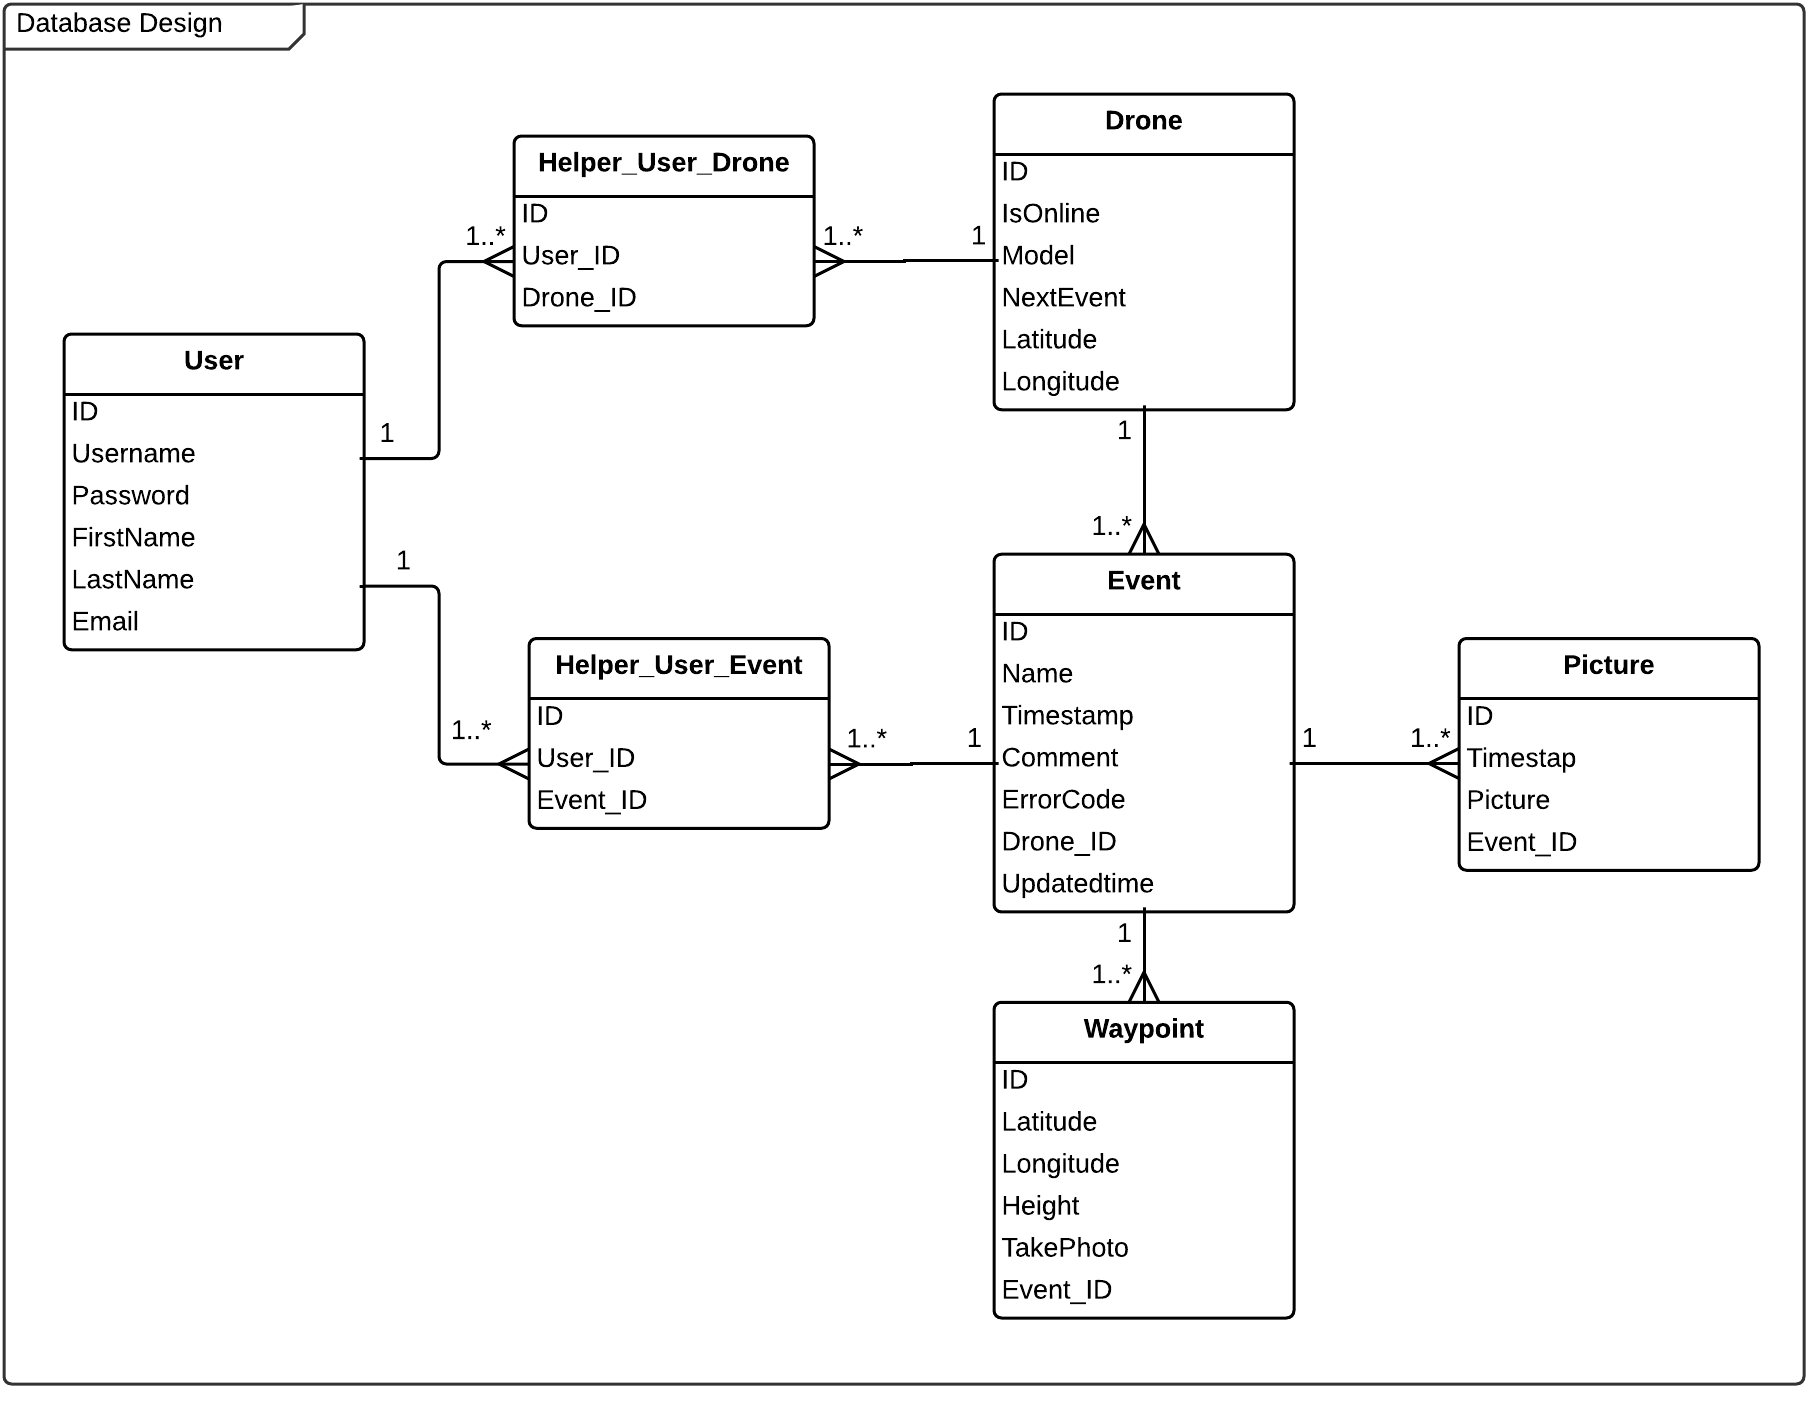
\includegraphics[width=1\textwidth]{Billeder/database/database_design.png}
	\vspace{-.5cm}
	\caption{Database design}
	\label{fig:database_design}
\end{figure}


\newpage
\subsubsection*{Tilgængelige endpoints}
De tilgængelige endpoint i API'et er følgende:

\begin{table}[H]
\begin{tabular}{| p{3cm}| p{11.5cm}|}
\hline
Endpoint:	 							& \textbf{\textit{api/waypoints/}}\\\hline
Allows:									& POST, OPTIONS, GET\\\hline
Content-Type:						& application/json\\\hline 
Indehold:								& Giver adgang til waypoints tabellen, med muglighed for at tilføje nye waypoints\\\hline 
Kommentar:							& Det er muligt at tilføje "?format=json" til URL'en for at få dataen i ren json format\\\hline
\end{tabular}
\caption{Waypoint endpoint}
\label{waypoint_endpoint}
\end{table}

\begin{table}[H]
\begin{tabular}{| p{3cm}| p{11.5cm}|}
\hline
Endpoint:	 							& \textbf{\textit{api/users/}} \\\hline
Allows:									& OPTIONS, GET\\\hline
Content-Type:						& application/json\\\hline 
Indehold:								& Giver adgang til user tabellen\\\hline 
Kommentar:							& Det er muligt at tilføje "?format=json" til URL'en for at få dataen i ren json format\\\hline
\end{tabular}
\caption{User endpoint}
\label{user_endpoint}
\end{table}

\begin{table}[H]
\begin{tabular}{| p{3cm}| p{11.5cm}|}
\hline
Endpoint:	 							&\textbf{\textit{api/pictures/}} \\\hline
Allows:									& POST, OPTIONS, GET\\\hline
Content-Type:						& application/json\\\hline 
Indehold:								& Giver adgang til pictures tabellen, med mulighed for at tilføje nye billeder\\\hline 
Kommentar:							& Det er muligt at tilføje "?format=json" til URL'en for at få dataen i ren json format\\\hline
\end{tabular}
\caption{Picture endpoint}
\label{picture_endpoint}
\end{table}

\begin{table}[H]
\begin{tabular}{| p{3cm}| p{11.5cm}|}
\hline
Endpoint:	 							&\textbf{\textit{api/events/}}\\\hline
Allows:									& POST, PUT, OPTIONS, GET\\\hline
Content-Type:						& application/json\\\hline 
Indehold:								& Giver adgang til event tabellen, med mulighed for at oprette nye events og opdatere dem\\\hline 
Kommentar:							& Det er muligt at tilføje "?format=json" til URL'en for at få dataen i ren json format\\\hline
\end{tabular}
\caption{Event endpoint}
\label{event_endpoint}
\end{table}

\begin{table}[H]
\begin{tabular}{| p{3cm}| p{11.5cm}|}
\hline
Endpoint:	 							&\textbf{\textit{api/drones/}}\\\hline
Allows:									& POST, OPTIONS, GET\\\hline
Content-Type:						& application/json\\\hline 
Indehold:								& Giver adgang til drone tabellen, med mulighed for at tilføje nye droner\\\hline 
Kommentar:							& Det er muligt at tilføje "?format=json" til URL'en for at få dataen i ren json format\\\hline
\end{tabular}
\caption{Drones endpoint}
\label{drones_endpoint}
\end{table}

\begin{table}[H]
\begin{tabular}{| p{3cm}| p{11.5cm}|}
\hline
Endpoint:	 							&\textbf{\textit{api/drones/\#/}}\\\hline
Allows:									& PUT, OPTIONS, GET\\\hline
Content-Type:						& application/json\\\hline 
Indehold:								& Giver adgang til en record i drone tabellen, med mulighed for at opdatere droner\\\hline 
Kommentar:							& Det er muligt at tilføje "?format=json" til URL'en for at få dataen i ren json format\\\hline
\end{tabular}
\caption{Single drone endpoint}
\label{single_drone_endpoint}
\end{table}

\newpage
\subsection{Detaljeret database beskrivelse}

\subsubsection*{User table}
Tabellen indeholder data om systemets brugere. Tabellen gør det via Foring keys muligt for systemets brugere at tilgå droner, events og de gemte flyruter i systemet.
\vspace{-5pt}
\begin{figure}[H]
	\centering
	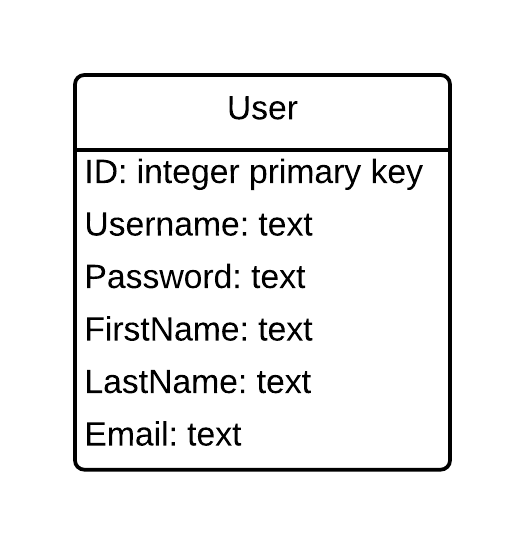
\includegraphics[width=0.5\textwidth]{Billeder/database/UserTabel.png}
	\vspace{-5pt}
	\caption{User table}
	\label{fig:user_table}
\end{figure}

\begin{table}[H]
\begin{tabular}{| p{3cm}| p{11.5cm}|}
\hline

Formål	 							& At holde data om brugere i systemet, samt tjekke om brugere eksisterer, når de forsøger at logge på webapplikation.\\\hline
Forbindelser						& Tabellen har en foreing key til at hjælpe tabellerne: Helper User Drone og Helper User Event.\\\hline
Attributter						& \begin{itemize}
												\item ID: Primary key.
												\item Username: Brugernavnet til systemet. Max length: 50 char
												\item Password: Brugerens kode. Max length: 50 char
												\item FirstName: Brugers fornavn. Max length: 50 char
												\item LastName: Brugerens efternavn. Max length: 50 char
												\item Email: Brugerens email adresse.
											\end{itemize} \\\hline 
\end{tabular}
\caption{User table}
\label{tab:user_table}
\end{table}
\newpage
\subsubsection{Event table}
Tabellen indeholder data om events i systemet. Tabellen fungere som omdrejnings punkt i databasen. Droner kan tilkobles et event, billeder bliver tilføjet til et event og waypoints bliver tilføjet til et event.
\vspace{-5pt}
\begin{figure}[H]
	\centering
	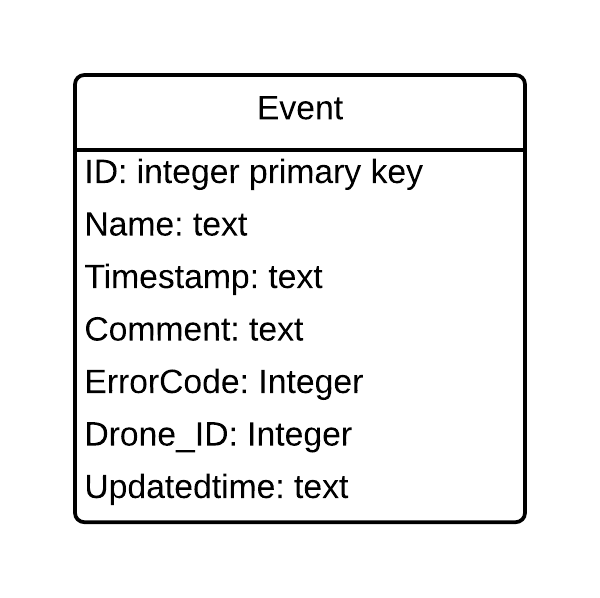
\includegraphics[width=0.5\textwidth]{Billeder/database/EventTable.png}
	\vspace{-5pt}
	\caption{Event table}
	\label{fig:event_table}
\end{figure}

\begin{table}[H]
\begin{tabular}{| p{3cm}| p{11.5cm}|}
\hline

Formål	 							& Holde data om events i systemet.\\\hline
Forbindelser						& Tabellen har en foreing key til user tabellen med en mange til mange relation. Drone-, waypoint- og picture-tabellen har foreing keys til tabellen.\\\hline
Attributter						& \begin{itemize}
												\item ID: Primary key.
												\item Name: Navnet på det givet event. Max length: 100 char
												\item Timestamp: Timestamp for oprettelse: Datefield
												\item Updated: Timestamp for opdaterede: Datefield
												\item Comment: Kommentar til givet event. Max length: 100 char
												\item ErrorCode: Fejlkode hvis fejl opstår under flyvning: Integer
												\item UserId: Mange til mange relation til user tabellen: Foreingkey
											\end{itemize} \\\hline 
\end{tabular}
\caption{Event table}
\label{tab:event_table}
\end{table}
\newpage
\subsubsection{Picture table}
Tabellen indeholder data om billeder taget af dronen i systemet, samt selve billederne. Billeder bliver gemt i en blob type, som bare er binær-data i databasen.
\vspace{-5pt}
\begin{figure}[H]
	\centering
	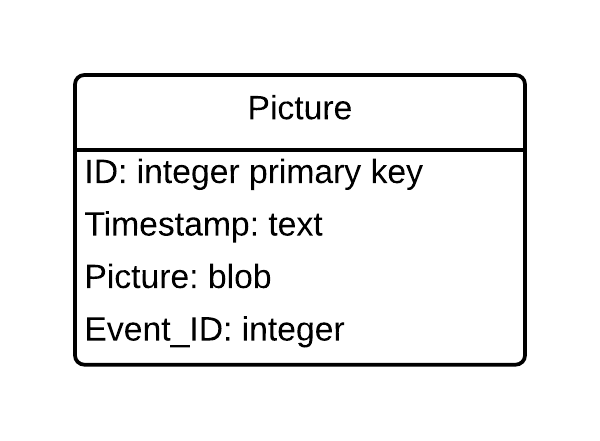
\includegraphics[width=0.5\textwidth]{Billeder/database/PictureTable.png}
	\vspace{-5pt}
	\caption{Picture table}
	\label{fig:picture_table}
\end{figure}

\begin{table}[H]
\begin{tabular}{| p{3cm}| p{11.5cm}|}
\hline

Formål	 							& Holde data om billeder i systemet og selve billederne.\\\hline
Forbindelser						& Tabellen har en foreing key til event tabllen.\\\hline
Attributter						& \begin{itemize}
												\item ID: Primary key.
												\item Name: Navnet på det givet event. Max length: 100 char
												\item Timestamp: Timestamp for oprettelse: Datefield
												\item Picture: blob: Udefinerbar størrelse binær data
												\item Event ID: Relation til event tabellen: Foreingkey
											\end{itemize} \\\hline 
\end{tabular}
\caption{Picture table}
\label{tab:picture_table}
\end{table}
\newpage
\subsubsection*{Waypoint table}
Tabellen indeholder alle waypoints som brugeren har oprettet i systemet. Hvert waypoint i tabellen indeholder information om gps-koordinatet, højden og om der skal tages et billede ved lokationen eller ej.
\vspace{-5pt}
\begin{figure}[H]
	\centering
	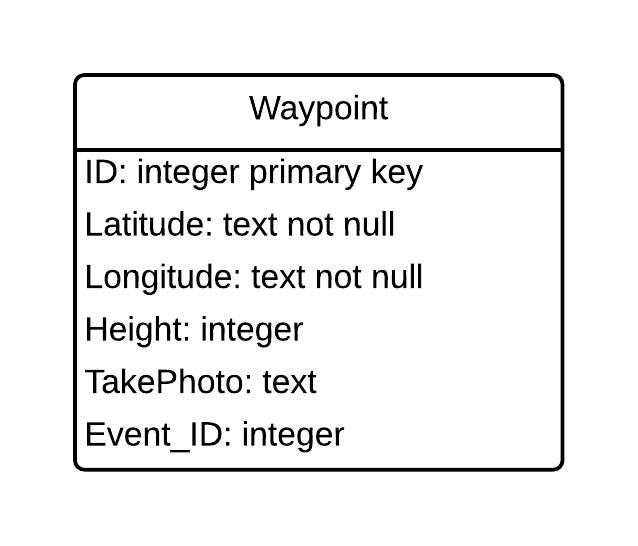
\includegraphics[width=0.5\textwidth]{Billeder/database/WaypointTable.png}
	\vspace{-5pt}
	\caption{Waypoint table}
	\label{fig:waypoint_table}
\end{figure}

\begin{table}[H]
\begin{tabular}{| p{3cm}| p{11.5cm}|}
\hline

Formål	 							& Holde data om waypoints i systemet.\\\hline
Forbindelser						& Waypoint tabellen har en foreing key til event tabellen.\\\hline
Attributter						& \begin{itemize}
												\item ID: Primary key.
												\item Latitude: Requried text felt. Max length: 100 char
												\item Longitude: Requried text felt. Max length: 100 char
												\item Height: Integer
												\item Event ID: Relation til event tabellen: Foreing key
											\end{itemize} \\\hline 
\end{tabular}
\caption{Waypoint table}
\label{tab:waypoint_table}
\end{table}
\newpage
\subsubsection*{Drone table}
Tabellen indeholder alle droner som er oprettet i systemet. Bruger har mulighed for at tilføje flere droner.
\vspace{-5pt}
\begin{figure}[H]
	\centering
	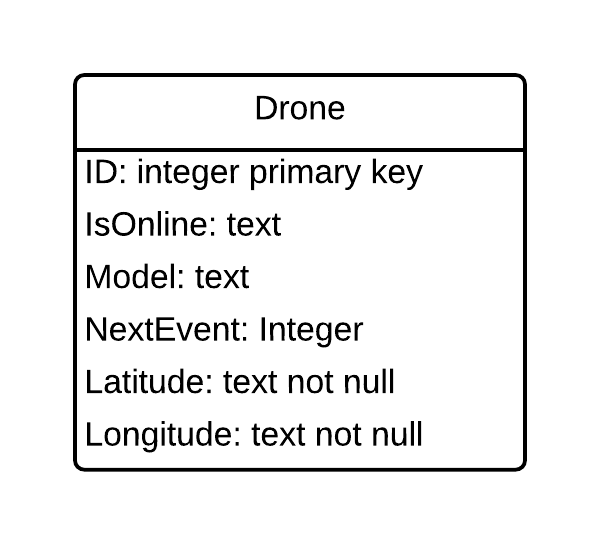
\includegraphics[width=0.5\textwidth]{Billeder/database/DroneTable.png}
	\vspace{-5pt}
	\caption{Drone table}
	\label{fig:drone_table}
\end{figure}

\begin{table}[H]
\begin{tabular}{| p{3cm}| p{11.5cm}|}
\hline

Formål	 							& Holde information om hver drone i systemet.\\\hline
Forbindelser						& Drone tabellen har en foreing key til event tabellen.\\\hline
Attributter						& \begin{itemize}
												\item ID: Primary key.
												\item IsOnline: Status for dronen: Boolean værdig
												\item Model: Modeltype: Text field: Max length 50 char
												\item NextEvent: Events for dronen: Integer field
												\item Latitude: Dronens GPS lokation: Max length 100 char  
												\item Longitude: Dronens GPS lokation: Max length 100 char
											\end{itemize} \\\hline 
\end{tabular}
\caption{Drone table}
\label{tab:drone_table}
\end{table}

